Para el análisis de los resultados de la recolección de datos utilizamos
diversos métodos. En primer lugar, tomamos la red como una fuente de
información y las IPs como símbolo. Usando esto como modelo, calculamos la
entropía de las redes invesigadas, usando tanto las ips de los receptores como
las de los emisores de los paquetes ARP. Otro modelo de información posible,
que también nos permitiría caracterizar los nodos de la red y su frecuencia
relativa de aparición, sería utilizar como símbolos las direcciones MAC de los
paquetes, y para esto debieramos haber guardado esta información al hacer las capturas. Esto nos da otro tipo de información, porque muchas veces pueden ser
distintos 

Luego, para tener una mejor visualización de los datos obtenidos, decidimos
utilizar diferentes gráficos para sintetizar y presentar la información que
consideramos más relevante de las redes analizadas.

En primer lugar usamos gráficos de torta para representar la proporción de
apariciones entre las IPs, discriminado por emisores y receptores. Sin embargo,
cuando el número de IPs distintas crecía (en particular con las redes de la
facultad) este método dejaba de ser eficiente porque el gráfico se volvía
incomprensible. Es por esto que en estos gráficos mostramos una versión
``reducida'' de las capturas.

En segundo lugar, usamos gráficos de barras para analizar la frecuencia
absoluta y relativa de aparición de cada una de las IPs, contando por separado
los paquetes en los que la IP era emisora y receptora.

Por último, usamos un histograma en 2 dimensiones con una escala cromática
que indica por cada par de IPs ($x$, $y$) la cantidad de paquetes ARP que se enviaron con origen $x$ y destino $y$.

Para ahorrar espacio con el texto de los gráficos, en todos los casos salvo los
gráficos de torta las IPs se expresan incompletas (solo los últimos 8 bits, que
son los que cambian). La primera parte en el caso de los laboratorios de la
facultad es siempre ``10.2.100'' y en la del trabajo de nuestro compañero
``10.10.99''.

Los resultados y análisis se exponen a continuación.


\subsection{Laboratorios del DC}

Con un total de 200 paquetes ARP capturados, obtuvimos una entropía en los
emisores de 2.81763365265 y en los receptores de 4.20465276111.

\subsubsection{Análisis de entropía}
Una primera observación que podemos hacer es que la entropía de los receptores es significativamente mayor que la de los emisores. Esto quiere decir que hay más incertidumbre en quién va a ser receptor que en quién va a ser emisor, esto probablemente se deba a que hay menos nodos que funcionan como emisores en comparación con los que funcionan como receptores, o que hay un conjunto reducido de nodos que tienen una alta probabilidad de ser emisores.
Las figuras \ref{fig:torta-emisor-facu} y \ref{fig:torta-receptor-facu} nos permiten aclarar un poco más estas hipótesis. Vemos que más de la mitad de los paquetes ARP tiene como origen a la IP 254, y el resto del espectro (un poco menos de la mitad) está dividido en las IPs restantes con una pequeña preponderancia de algunas. En cambio la distribución de las IP destino es totalmente fragmentada. Si bien la IP 254 sigue siendo la mayoritaria no tiene la mayoría del espectro, que se acerca a una división más equitativa que las IPs origen. El hecho de que la distribución de IPs origen sea más equitativa hace que el nivel de incertidumbre (y por tanto su entropía) sea mayor, recordemos que la entropía máxima se alcanza con una distribución equiprobable de los simbolos.

Más adelante, junto con la información que nos brindan los otros gráficos, vemos que correlato tiene esté análisis ``abstracto'' de la entropía con la función que cumplen los nodos en la red.

\subsubsection{Análisis de capturas}
\begin{figure}[!h]
  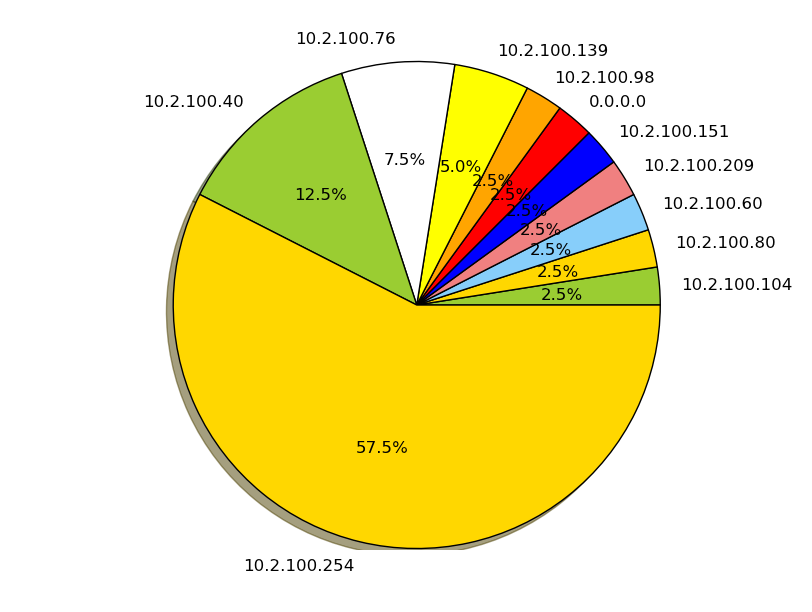
\includegraphics[width=\textwidth,keepaspectratio]{graph/emisores_facu.png}
  \caption{Proporción de IPs origen}
  \label{fig:torta-emisor-facu}
\end{figure}

\begin{figure}[!h]
  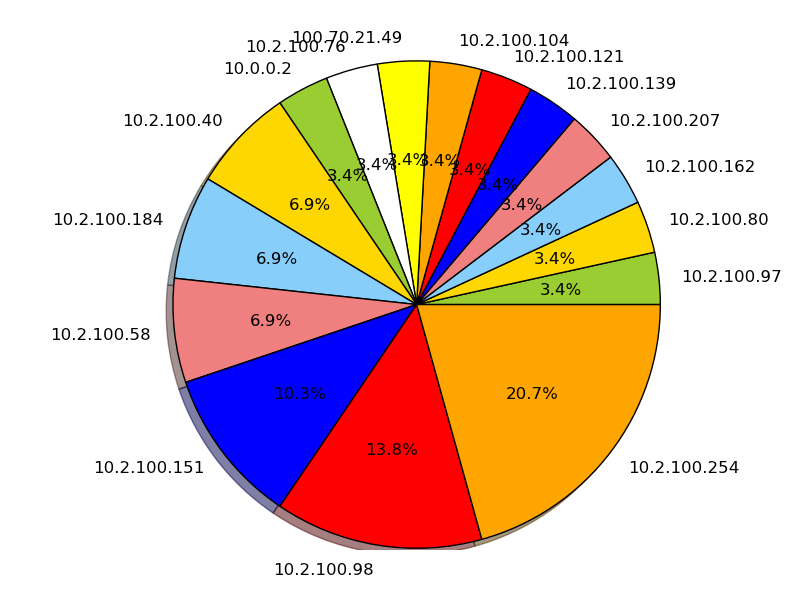
\includegraphics[width=\textwidth,keepaspectratio]{graph/receptores_facu.png}
  \caption{Proporción de IPs destino}
  \label{fig:torta-receptor-facu}
\end{figure}

\begin{figure}[!h]
  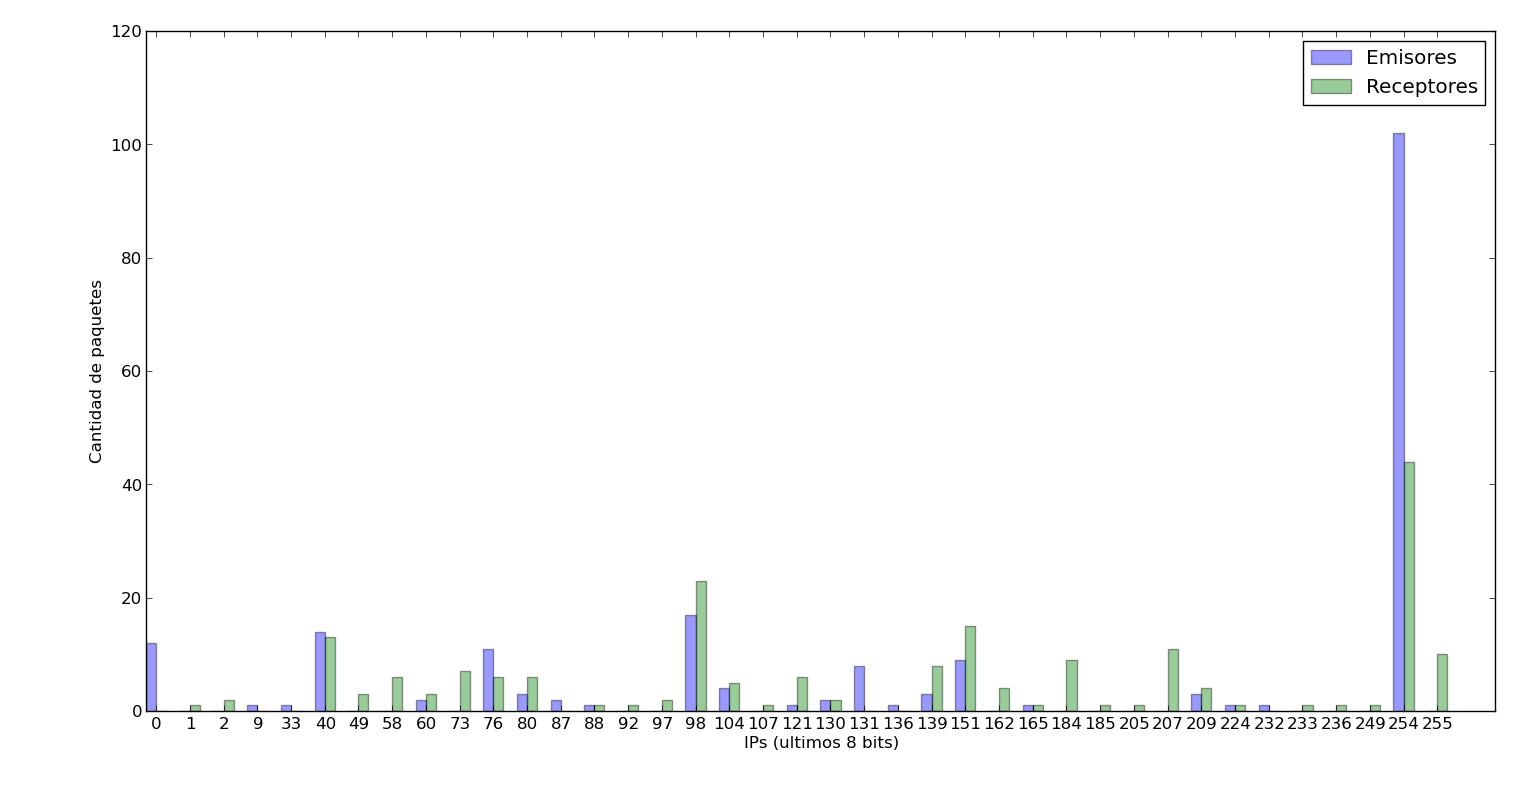
\includegraphics[width=\textwidth,keepaspectratio]{graph/barras-facu.png}
  \caption{Cantidad de paquetes por IP discriminados en emisores y receptores}
  \label{fig:barras-facu}
\end{figure}

\begin{figure}[!h]
  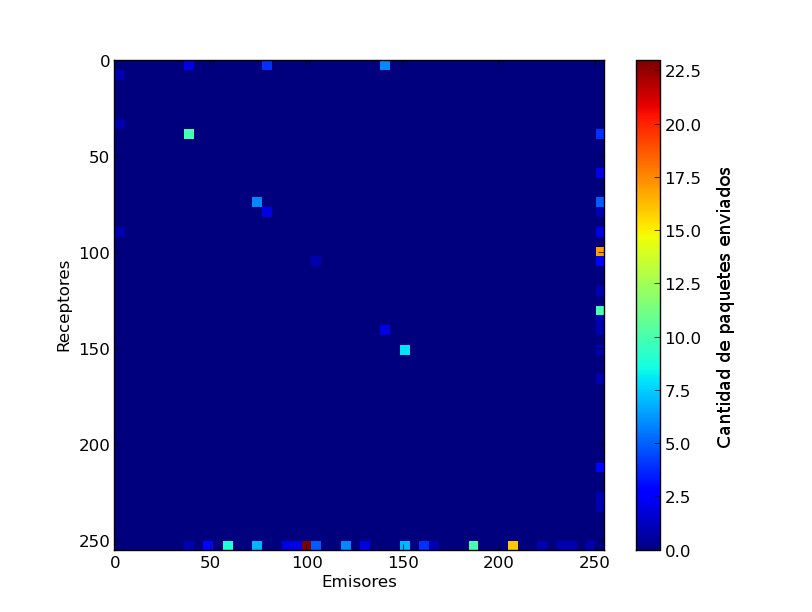
\includegraphics[width=\textwidth,keepaspectratio]{graph/hist2d-facu.png}
  \caption{Relación entre emisores y receptores}
  \label{fig:hist2d-facu}
\end{figure}

Como se puede observar claramente en los gráficos de torta y la figura
\ref{fig:barras-facu}, hay una gran presencia del dispositivo con la IP
10.2.100.254, seguido de lejos por la 10.2.100.98. El dispositivo 254 genera muchas más solicitudes de las que recibe, esto podemos verlo en los gr\'aficos de tortas y en el gr\'afico de barras.

La relaci\'on entre estos dos nodos m\'as importantes se puede aclarar con la figura \ref{fig:hist2d-facu}, donde se
aprecia que 10.2.100.98 prácticamente solo pregunta por 10.2.100.254 y es el que genera la mayor parte de las solicitudes al 254.
También en el histograma en se puede visualizar en los margenes derecho e inferior que 10.2.100.254 pregunta por
varias IPs distintas y también es consultado por varias otras, lo que nos indica que en en esta dirección hay un dispositivo muy solicitado. Otra observación,
bastante extraña por cierto, es que hay cierta tendencia de algunos dispositivos
a preguntar por ellos mismos (por eso la clara diagonal del histograma).

En las figuras \ref{fig:barras-facu} y \ref{fig:hist2d-facu} se observa
que la mayor parte de las IPs disponibles (tomando en cuenta solo las que
comienzan por ``10.2.100'') fueron usadas en algún momento de la captura.

En contadas ocasiones (apreciables tanto en el dump de la captura
como en las figuras \ref{fig:barras-facu} y \ref{fig:hist2d-facu}), apareció la
IP 0.0.0.0 (la única que no comienza con ``10.2.100'') como emisora de
solicitudes ARP con distintos destinos. Investigando un poco, descubrimos que
esta es una IP que se utiliza para dispositivos que no están conectados a
ninguna red TCP/IP. Es también una IP ficticia que se usa para representar
direcciones inválidas, a menudo impresoras mal configuradas, paquetes con emisor
desconocido, o cuando DHCP falla o tarda demasiado tiempo.

También descubrimos que, salvo por las consultas autorreferenciales y las que
involucran a 10.2.100.254 y a 0.0.0.0, las consultas entre nodos distintos son
inexistentes.

Adelantando una de las conclusiones, probablemente el router de la red se encuentra en el nodo 254. Y esto nos termina de aclarar el análisis de entropía, ya que debido a que hay una alta actividad del router por redirigir paquetes a los nodos internos de la red hegemoniza la mayor parte de las emisiones de paquetes ARP. Y es por esto que hay menos incertidumbre en las emisiones.

A raíz de estas observaciones, podemos concluir algunas cosas:
\begin{itemize}
  \item El router de la red seguramente se encuentra en 10.2.100.254, y
probablemente sea el nodo de salida a Internet.
  \item En 10.2.100.98 probablemente haya un dispositivo que estaba configurado
para renovar sus tablas ARP en intervalos cortos.
  \item Hay ocasiones en las que DHCP falla y deja dispositivos sin IP, o bien
hay dispositivos enviando paquetes con IPs emisoras inválidas o secretos. En
cualquier caso, esto arruina la función de ARP, ya que nadie puede
responder a una IP que no es ruteable.
  \item Por momentos los dispositivos tienen leves síntomas de
esquizofrenia.
  \item Más allá de las preguntas por sí mismos y las consultas al router, no
existen consultas entre dispositivos. Mientras duró la captura ninguno de ellos
trató de comunicarse con otro.
  \item Todo esto nos lleva a pensar que la función principal de la red es
proveer de salida a Internet a los dispositivos que se conecten a ella, más que
permitirles la comunicación directa entre dispositivos de la misma red.
  \item La cantidad de dispositivos conectados a la red es grande.  Esto podría
explicar la sobrecarga del servidor de DHCP, que falla o tarda mucho tiempo en
asignar IPs a los nuevos dispositivos. 
\end{itemize}

\newpage
\subsection{Oficinas de InvGate}
Con un total de 11158 paquetes ARP capturados, obtuvimos una entropía en los
emisores de 2.85760098357 y en los receptores de 3.08636573523.

\subsubsection{Análisis de entropía}
En este caso no hay una diferencia significativa del valor de la entropía entre IPs origen e IPs destino. Pero así como anteriormente contrastamos estos valores con los gráficos podemos hacer lo propio con este caso. En el gráfico de IPs origen vemos que básicamente la mitad del espectro está acaparada por una computadora y la otra mitad está distribuida sin una clara preponderancia de alguna IP en particular. En cambio la distribución del las IPs destino se presenta fragmentada en más areas grandes. Gran parte del espectro se divide de manera equitativa entre algunas pocas IPs. 
Por un lado la distribución de IPs origen presenta un 50\% dividido en pequeños pedazos, lo que indicaría un nivel de incertidumbre mayor a las ``areas grandes'' que presentan las IPs destino. Pero por otro lado estas últimas logran fragmentar, aunque sea en pocas IPs, lo que en el gráfico de IPs origen se presenta como un bloque de una única IP.
Al parecer está pesando más este segundo análisis en el cálculo de la entropía, y por eso la de receptores es mayor.

Más adelante vemos que el hecho de que la cantidad de información de receptores es similar a la de emisores está intimamente relacionado con la función que cumplen los nodos en la red.

\subsubsection{Análisis de capturas}
\begin{figure}[!h]
  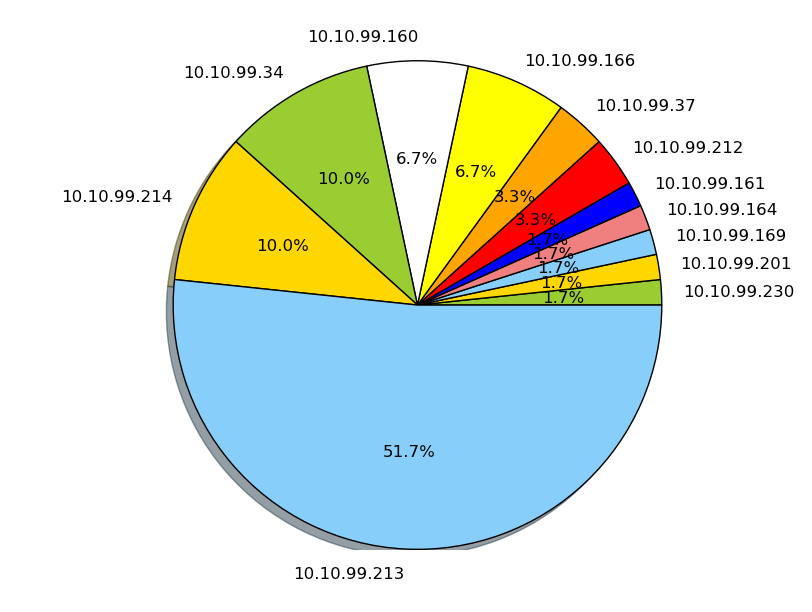
\includegraphics[width=\textwidth,keepaspectratio]{graph/emisores_somodi.png}
  \caption{Proporción de IPs origen}
  \label{fig:torta-emisor-inv}
\end{figure}

\begin{figure}[!h]
  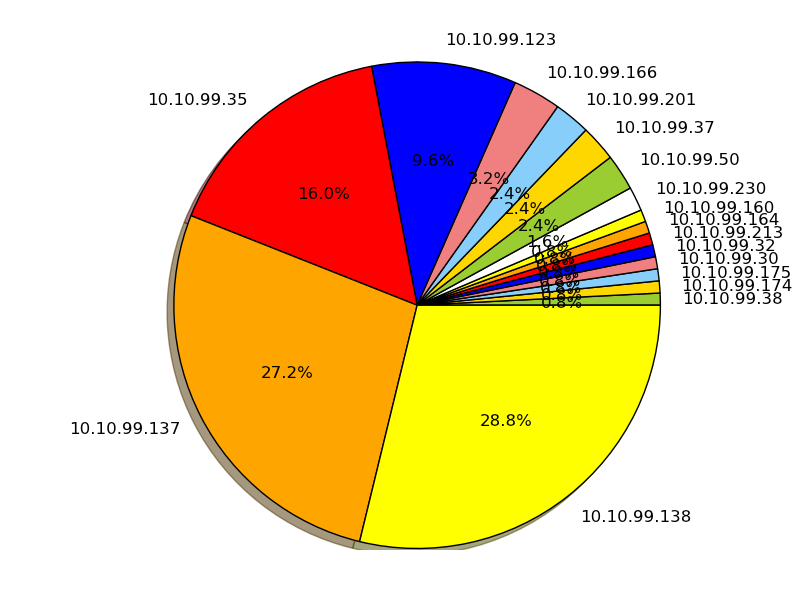
\includegraphics[width=\textwidth,keepaspectratio]{graph/receptores_somodi.png}
  \caption{Proporción de IPs destino}
  \label{fig:torta-receptor-inv}
\end{figure}

\begin{figure}[!h]
  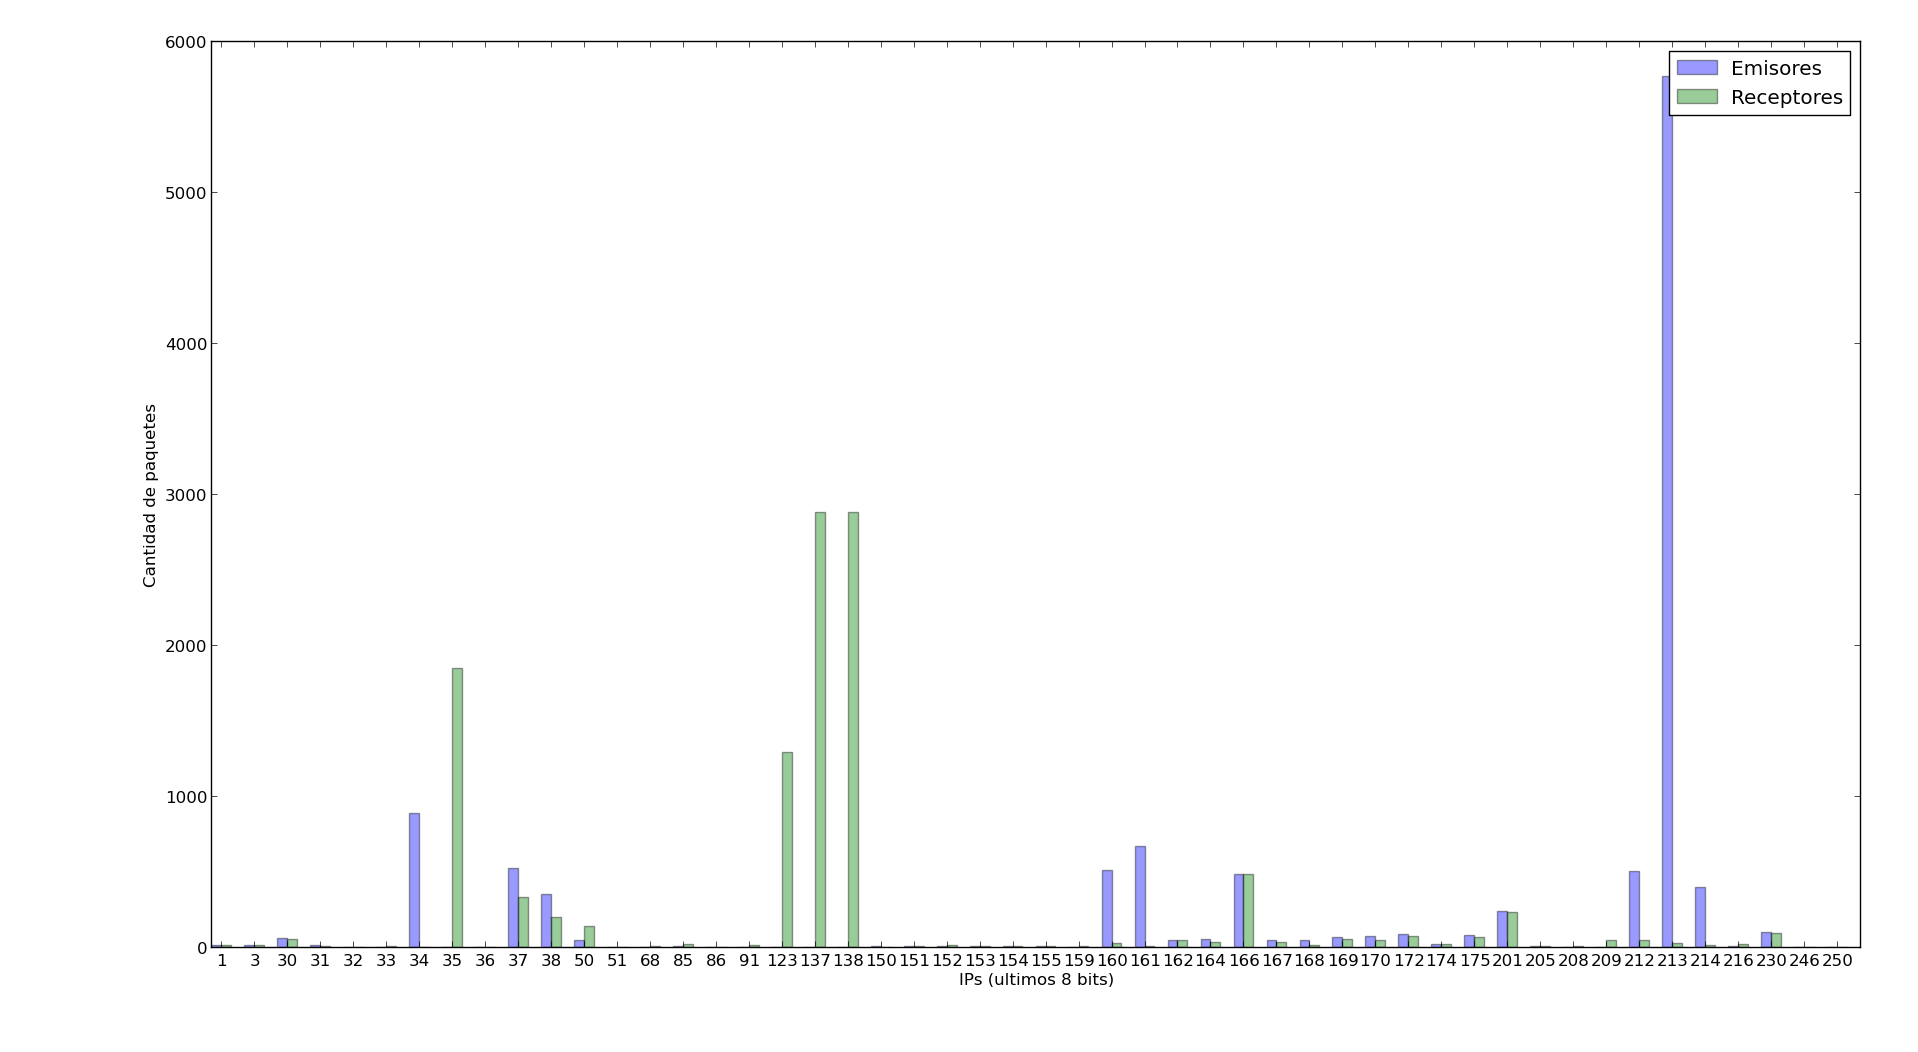
\includegraphics[width=\textwidth,keepaspectratio]{graph/barras-invgate.png}
  \caption{Cantidad de paquetes por IP discriminados en emisores y receptores}
  \label{fig:barras-inv}
\end{figure}

\begin{figure}[!h]
  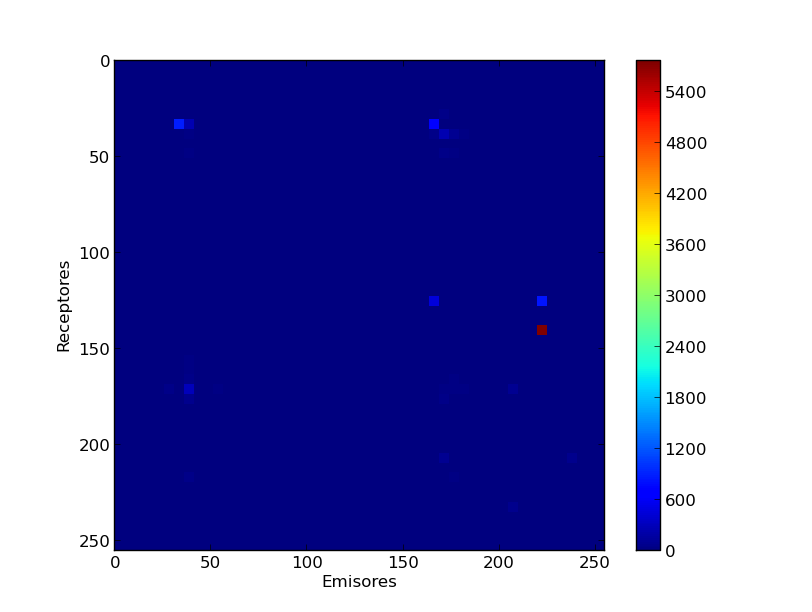
\includegraphics[width=\textwidth,keepaspectratio]{graph/hist2d-invgate.png}
  \caption{Relación entre emisores y receptores}
  \label{fig:hist2d-inv}
\end{figure}

Como se puede observar claramente en las figuras \ref{fig:torta-emisor-inv} y  
\ref{fig:barras-inv}, hay una gran presencia del dispositivo con la IP 10.10.99.213 cuyo comportamiento se limita a generar paquetes ARP y enviarlos. Como vemos en la figura \ref{fig:torta-receptor-inv} casi nunca es el destino de una consulta who-is. Por otro lado, a éste lo siguen dos dispositivos de igual cantidad de apariciones en los paquetes: las IPs 10.10.99.138 y 10.10.99.137. A diferencia del nodo 213, podemos ver en los gráficos de torta que estos nodos solo se encuentran como IPs destino, es decir, IPs por las cuales se consulta o se informa a qué MAC corresponde.

La figura \ref{fig:hist2d-inv} nos muestra la interacción de los nodos que tienen una cantidad de actividad considerable. Esto se debe a que la escala de cantidad de paquetes enviados llega a mas de 5400, con lo cual los nodos que no tengan una actividad en orden de cientos de paquetes no están reflejados. Esto no es un problema porque nos permite concentrar nuestra atención la interacción en aquellos nodos que tiene un rol activo en la red. Como vemos más adelante esta actividad no está concentrada solo en uno o un par de nodos.
Podemos ver la interacción que se corresponde con estos dispositivos. Vemos que casi la totalidad de los paquetes envíados por el dispositivo 213 están dirigidos a los dispositivos 137 y 138.  Contrastando esto con los datos de los paquetes capturados vemos que el dispositivo 213 envía constantemente paquetes who-is preguntando por las IP 137 y 138, pero no se obtiene ninguna respuesta.
Además de esto, el histograma nos muestra la interacción entre otros nodos de la red. El gráfico muestra al menos otros 5 nodos que son parte de esta interacción, lo interesante es que estos nodos no se conectan de manera centralizada.

Otros nodos que solo actuan de receptores de paquetes son el 35 y el 123. En la figura \ref{fig:hist2d-inv} y en el dump de capturas podemos ver que los que hacen peticiones sobre el nodo 135 son el nodo 34 y el 161. Y los que hacen peticiones sobre el 123 son el 212, 214 y 160.

A diferencia del experimento en los laboratorios del DC, vemos que en las oficinas de InvGate sí existen consultas entre nodos distintos, esto nos da una pauta de que el comportamiento de la red no está centralizado en un nodo particular, sino que está distribuido entre los nodos existentes. 

Este último análisis es consistente con que la entropía de emisores y receptores sea similar, ya que la actividad es descentralizada tanto en emisores como en receptores.

Por otro lado es necesario aclarar que los nodos de los que nunca se obtiene respuesta, como el 25, 123, 137 y 138 probablemente sean dispositivos que no existen.

A raíz de estas observaciones, podemos concluir algunas cosas:
\begin{itemize}
  \item O bien la red no provee de salida a Internet, o bien la salida a Internet está distribuida en diferentes nodos de la red, pues de no ser así veríamos una estructura más centralizada en un único nodo.
  \item Probablemente en algún momento hubo dispositivos en las IPs 10.10.99.25, 10.10.99.123, 10.10.99.137, 10.10.99.138, pero estos ya no forman parte de la red.
  \item Los dispositivos que aún pertenecen a la red, como el 213 o el 34 no parecen estar enterados que los otros dispositivos ya no existen.
  \item El dispositivo 213 parece estar configurado para conectarse con las IPs 10.10.99.137, 10.10.99.138, ya que constantemente intenta preguntar si algún dispositivo se encuentra en estas. Esto puede deberse por ejemplo a algun protocolo que quedó configurado en el dispositivo, que redirige el tráfico de cierto puerto a esas IPs.
  \item Todo esto nos lleva a pensar que la función de la red es más compleja que simplemente proveer Internet. Probablemente se trate de varios dispositivos que cumplen cada uno una función particular y se interrelacionan, como por ejemplo computadoras de trabajo, impresoras que reciben información de estas computadoras, dispositivos móviles.
  \item Esta hipótesis parece llevarse bien con el hecho de que la red elegida pertenece a un lugar de trabajo de desarrollo de software.
\end{itemize}

